\begin{frame}{Безынерционная модель}
    \begin{itemize}
    \item {
        Экипаж состоит только из платформы и $N$ дисков колес.
    }
    \item {
        Количество твердых тел $1 + N$.
    }
    \item {
        Связи: для каждого колеса задан вектор $\vec{e}_i$, составляющий постоянный угол $\psi$ с плоскостью колеса, и для точек $C_i$ контакта:
        \vspace{-15pt}
        $$\vec{v}_{C_i} \cdot \vec{e}_i = 0$$
    }
    \end{itemize}
    \vspace{-10pt}
    \begin{figure}[H]
        \centering
        \begin{columns}
            \column{0.45\textwidth}
                \centering
                % 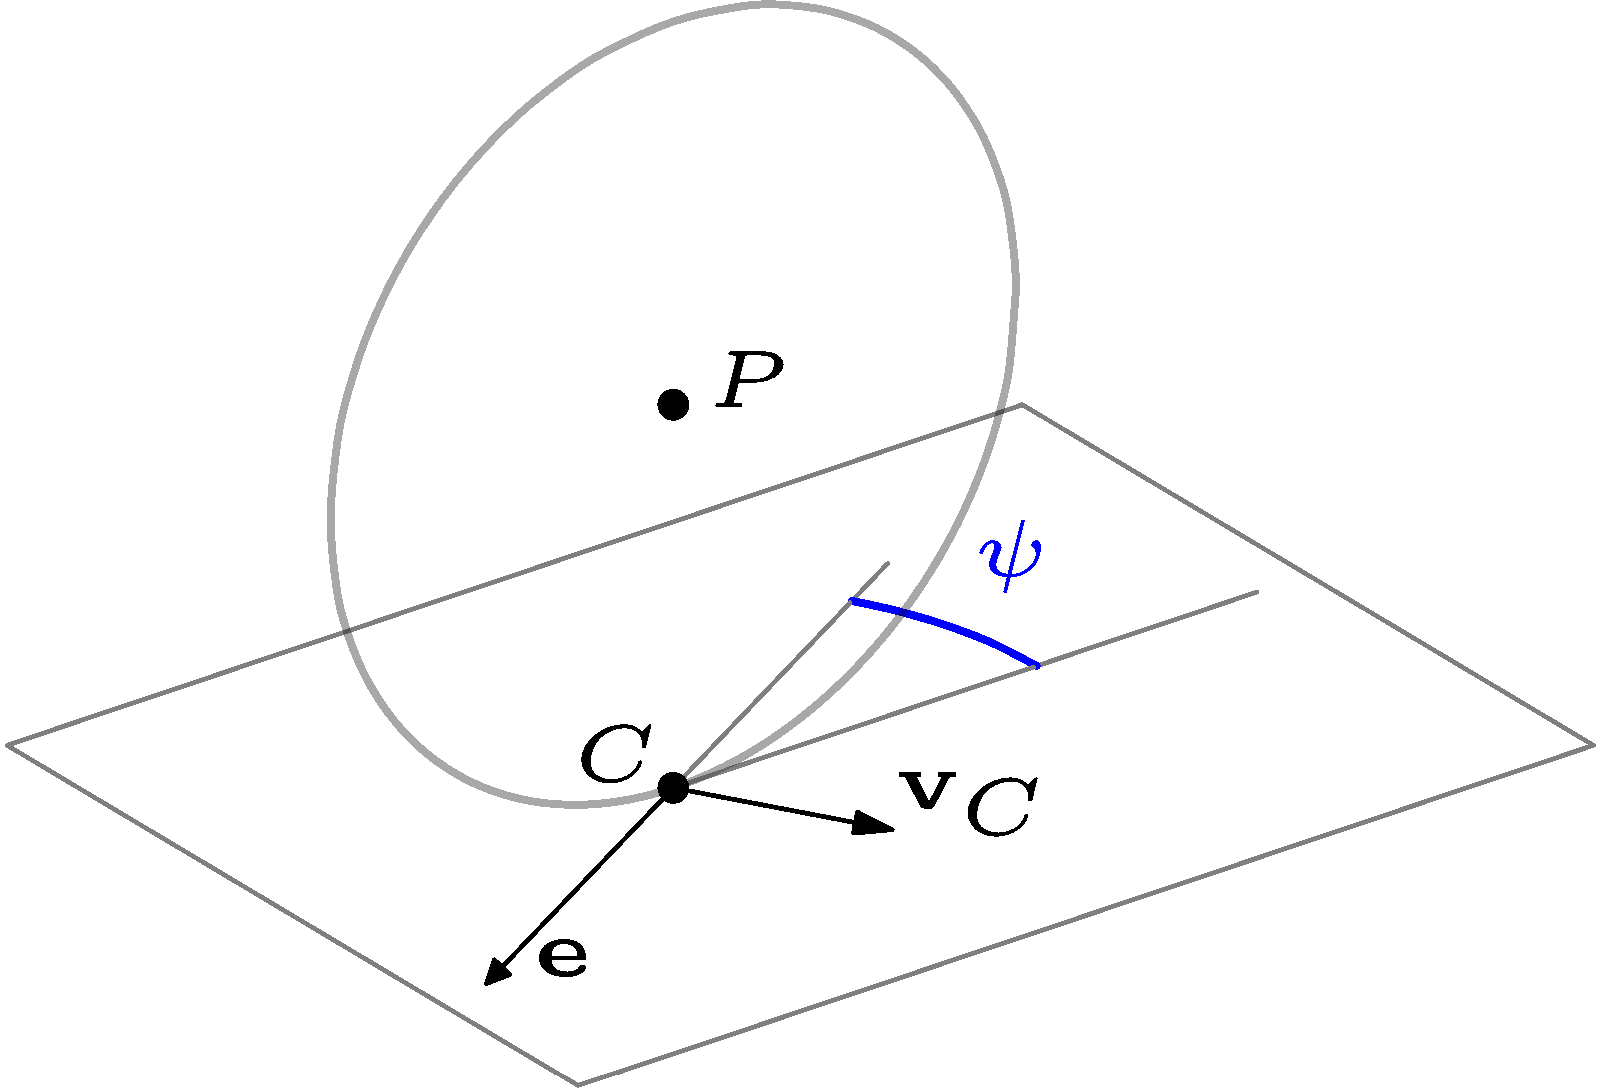
\includegraphics[width=\textwidth]{content/pic/asy/wheel_bor.png}
                \asyinclude[width=\textwidth]{content/pic/asy/wheel_bor.asy}
                \caption{Колесо}
                \label{fig:bor_wheel_scheme}
                % Рис.: Колесо \\
                % .
            \column{0.45\textwidth}
                \centering
                % 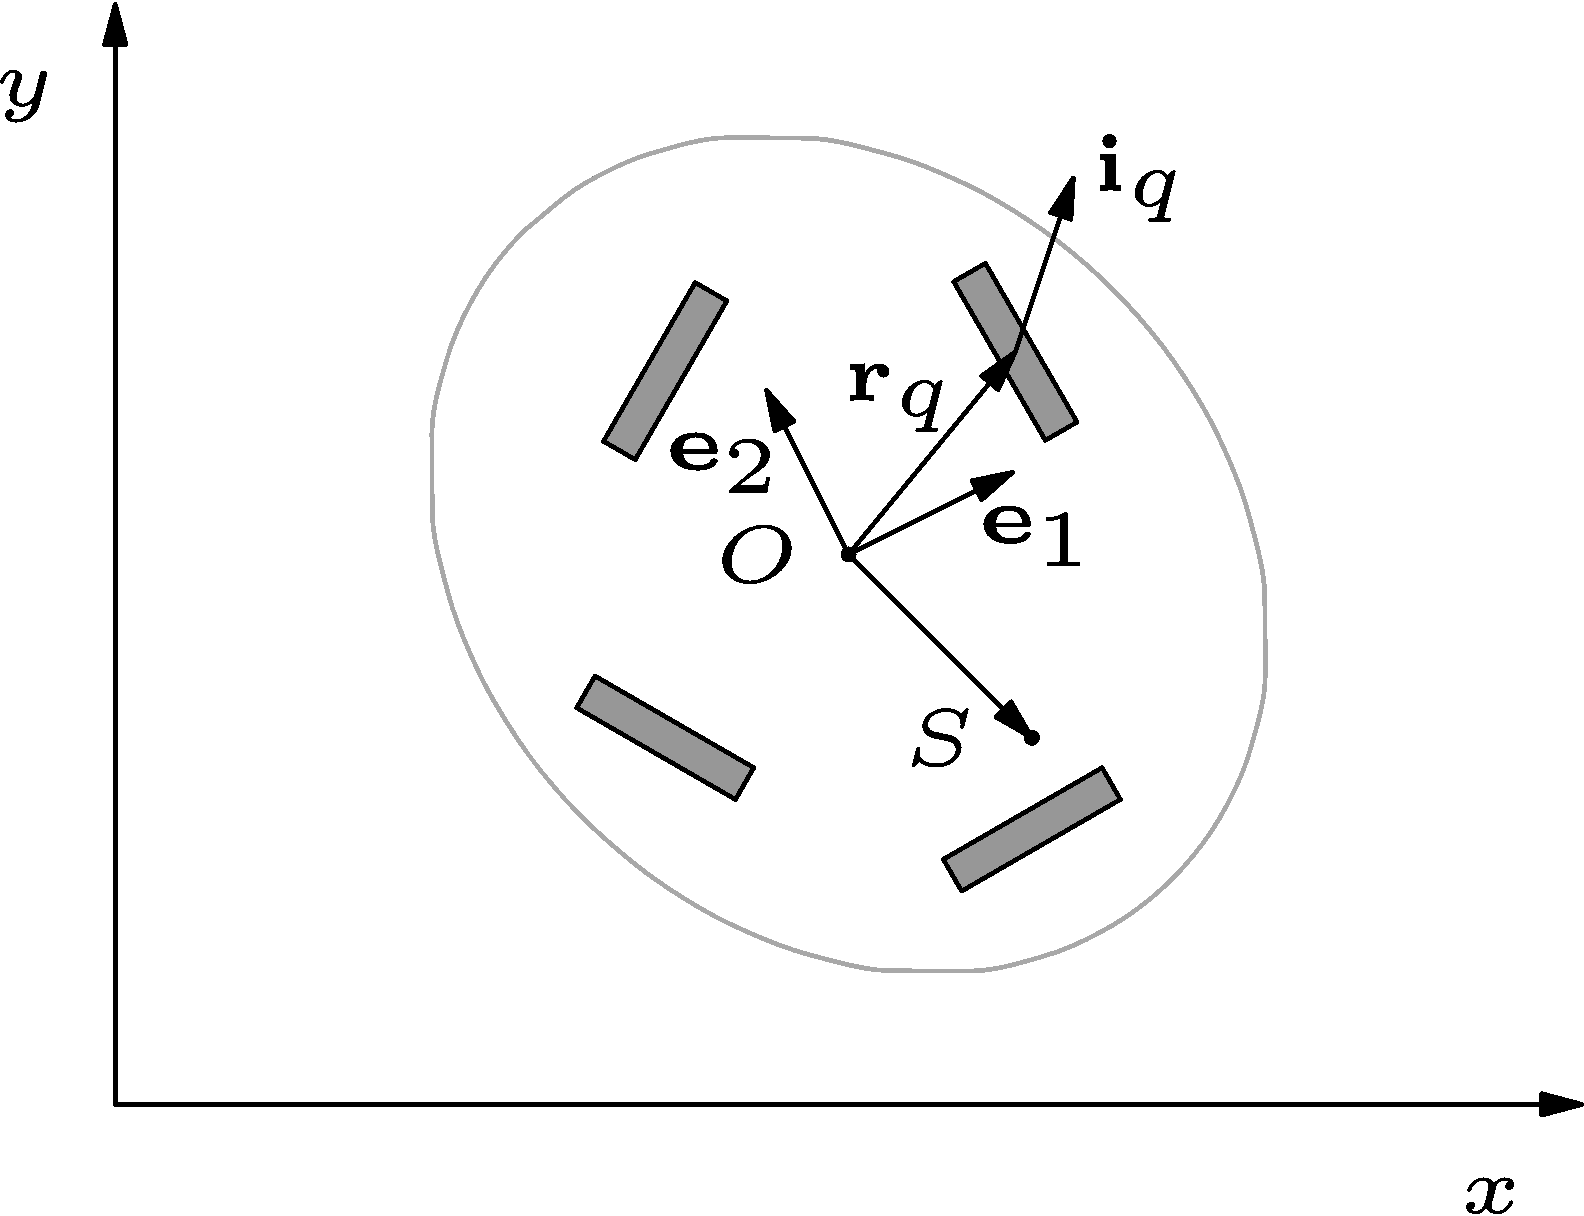
\includegraphics[width=\textwidth]{content/pic/asy/cart_bor.png}
                \asyinclude[width=\textwidth]{content/pic/asy/cart_bor.asy}
                \caption{Экипаж}
                \label{fig:bor_vehicle}
                % Рис.: Экипаж
        \end{columns}
    \end{figure}
\end{frame}